\documentclass{sig-alternate}

\usepackage{url}
\usepackage{graphicx}

\newcommand{\nPrograms}{250,166}
\newcommand{\nAnalyzedPrograms}{247,798}
\newcommand{\nemptyPrograms}{14,307}
\newcommand{\nScriptPrograms}{233,491}
\newcommand{\nLOC}{36,085,654}
\newcommand{\nscripts}{4,049,356}

\newcommand{\todo}[1]{\textbf{#1}}

\begin{document}
%
% --- Author Metadata here ---
%\conferenceinfo{WOODSTOCK}{'97 El Paso, Texas USA}
% --- End of Author Metadata ---

\title{How Kids Code and How We Know:\\An Exploratory Study on the Scratch Repository }

\numberofauthors{1}
\author{
% 1st. author
\alignauthor
(anonymized submission)
%Ben Trovato\titlenote{Dr.~Trovato insisted his name be first.}\\
%       \affaddr{Institute for Clarity in Documentation}\\
%       \affaddr{1932 Wallamaloo Lane}\\
%       \affaddr{Wallamaloo, New Zealand}\\
%       \email{trovato@corporation.com}
% 2nd. author
%\alignauthor
%G.K.M. Tobin\titlenote{The secretary disavows
%any knowledge of this author's actions.}\\
%       \affaddr{Institute for Clarity in Documentation}\\
%       \affaddr{P.O. Box 1212}\\
%       \affaddr{Dublin, Ohio 43017-6221}\\
%       \email{webmaster@marysville-ohio.com}
}

%\date{30 July 1999}

\maketitle
\begin{abstract}
Block-based programming languages like Scratch, Alice and Blockly are becoming increasingly common as introductory languages in programming education. There is substantial research showing that these visual programming environments are suitable for teaching programming concepts. But, what do people do when they use Scratch? In this paper we explore the characteristics of Scratch programs. To this end we have scraped the Scratch public repository and retrieved 250.000 projects. We present an analysis of these projects in three different dimensions. Initially, we look at the types of blocks used and the size of the projects. We then investigate complexity, used abstractions and programming concepts. Finally we detect \emph{code smells} like large scripts, dead code and duplicated code blocks. Our results show that 1) most Scratch programs are small, however Scratch programs consisting of over 100 sprites exist, 2) programming abstraction concepts like procedures are not commonly used and 3) Scratch programs do suffer from code smells including large scripts and unmatched broadcast signals.
\end{abstract}

% A category with the (minimum) three required fields
%\category{H.4}{Information Systems Applications}{Miscellaneous}
%A category including the fourth, optional field follows...
%\category{D.2.8}{Software Engineering}{Metrics}[complexity measures, performance measures]

\terms{terms}

\keywords{Scratch, programming practices, code smells, static analysis}

\section{Introduction}

Scratch \cite{resnick_scratch:_2009} is a programming language developed to teach children programming by enabling them to create games and interactive animations. The public repository of Scratch programs contains over 14 million projects. Scratch is a \emph{block-based} language: users manipulate blocks to program.

Block-based languages have existed since the eighties, but have recently found adoption as tools for programming education. In addition to Scratch, also Alice~\cite{conway_alice:_1994}, Blockly\footnote{\url{https://developers.google.com/blockly/}} and App Inventor~\cite{wolber_app_2011} are block-languages aimed at novice programmers.

Several studies have shown that block-based languages are powerful as tools for teaching programming~\cite{meerbaum-salant_learning_2010, b._moskal_evaluating_2005,cooper_teaching_2003,price_comparing_2015}. Previous work involving static analysis of Scratch programs have evaluated the application of various programming concepts in Scratch projects \cite{Maloney_2008,moreno_automatic_2014}. Recent works have focused on bad programming practices within Scratch programs \cite{Meerbaum_habits_2011}, and automated quality assessment tools have been proposed for identifying code smells~\cite{fowler_refactoring:_1999}~and bad programming practices \cite{boe_hairball:_2013,moreno_automatic_2014}. A recent controlled experiment found that long scripts and code duplication decreases a novice programmer's ability to understand and modify Scratch programs \cite{hermans_2016}.

The goal of this paper is to obtain a deep understanding of how people program in Scratch, to analyze the characteristics of Scratch programs, and to quantitatively evaluate the use of programming abstractions and concepts. Moreover, knowing that bad programming habits and code smells can be harmful \cite{hermans_2016}, we also want to explore whether they are common. To address this goal, we answer the following research questions:

\begin{itemize}
\item[RQ1] What are the size and complexity characteristics of Scratch programs?
\item[RQ2] Which coding abstractions and programming concepts and features are commonly used when programming in the Scratch environment?
\item[RQ3] How common are code smells in Scratch programs?
\end{itemize}

Our study is based on data from the Scratch project repository. By scraping the list of recent projects,\footnote{\label{scratchpublic}\url{https://scratch.mit.edu/explore/projects/all/}} we have obtained \nPrograms~public Scratch projects and performed source code analysis on them. To the best of our knowledge, this is the first large-scale exploratory study of Scratch projects.

The contributions of this paper are as follows:

\begin{itemize}
	\item{A public data set of \nScriptPrograms~non-empty Scratch projects (Section \ref{dataset})}
	\item{An evaluation of the data set in terms of size, complexity, programming concepts and smells (Section \ref{sec:results})}
	\item{A discussion of the implications of our findings for educational programming language designers (Section \ref{sec:discussion})}
\end{itemize}

\section{Relevant Scratch Concepts}
\label{sec:scratch}
This paper is by no means an introduction into Scratch programming, we refer the reader to \cite{brennan_creative_2014} for an extensive overview. To make this paper self-contained, however, we explain a number of relevant concepts in this section. 

Scratch is a block-based programming language aimed at children, developed by MIT. Scratch can be used to create games and interactive animations, and is available both as a stand-alone and as a web application. Figure \ref{fig:ui} shows the Scratch user interface. The main concepts in the Scratch programming environment are:

\begin{description}
	\item [Sprites] Scratch code is organized by `sprites': two dimensional pictures each having their own associated code. Scratch allows users to bring their sprites to life in various ways, for example by moving them in the plane, having them say or think words or sentences via text balloons, but also by having them make sounds, grow, shrink and switch costumes. The Scratch program in Figure \ref{fig:ui} contains two one sprites, the cat, which is Scratch's default sprite and a piano. The code in Sprite1 will cause the cat to move right when the right arrow is pressed, and when the green flag is clicked it will continuously sense touching the piano.
	\item [Scripts]Sprites can have multiple code blocks, called scripts. The Scratch code in Figure \ref{fig:ui} has two distinct scripts, one started by clicking on the green flag and one by pressing the space bar. It is possible for a single sprite to have multiple scripts initiated by the same event. In that case, all scripts will be executed simultaneously.
	\item [Events] Scratch is \emph{event-driven}: all motions, sounds and changes in the looks of sprites are initiated by events called Hat blocks\footnote{\url{http://wiki.scratch.mit.edu/wiki/Hat_Block}}). The canonical event is the \texttt{when Green Flag clicked}, activated by clicking the green flag at the top of the user interface. In addition to the green flag, there are a number of other events possible, including key presses, mouse clicks and input from a computer's microphone or webcam. The Scratch code in Sprite1 in Figure \ref{fig:ui} contains two events: \texttt{when Green Flag clicked} and \texttt{when <right arrow> key pressed}, each with associated blocks.
	\item [Signals] Events within Scratch can be user generated too: users can broadcast a message, for example when two sprites touch each other, like in Figure \ref{fig:ui}. All other sprites can then react by using the \texttt{when I receive} Hat block. In Figure \ref{fig:ui}, Sprite1 broadcasts `bump' when the cat touches the Piano. 
	\item[Custom blocks] Scratch users can define their own blocks, which users can name themselves, called custom blocks. The creation of custom blocks in Scratch is the equivalent of defining procedures in other languages \cite{moreno_automatic_2014}. Because the term `procedures' is common in related work, we will refer to custom blocks as `procedures' in the following. Procedures can have input parameters of type string, number, and boolean. When a user defines a procedure, a new Hat block called \texttt{define} appears, which users can fill with the implementation of their block.
\end{description}

\begin{figure}
	\begin{center}
		\includegraphics[width=\columnwidth]{fig/ui.png}
		\caption{The Scratch user interface consisting of the `cat' sprite on the left, the toolbox with available blocks in the category `Events' in the middle and the code associated with the sprite on the right.}
		\label{fig:ui}
	\end{center}
\end{figure} 

\section{Research design and dataset}
\label{researchDesign}

The main focus of this study is to understand how people program in Scratch by analyzing the characteristics of Scratch projects. To answer our three research questions, we conducted an empirical quantitative evaluation of project data we collected from the Scratch project repository. In the following paragraphs we describe the dataset, the process and the tools we used for analyzing it, and the methods we followed for detecting code smells.

\subsection{Dataset}
\label{dataset}

We obtained the set of Scratch projects by using a scraping program. Our scraping program called Kragle starts by reading the Scratch projects page\footnotemark[\ref{scratchpublic}] and thus obtains project ids of projects that were most recently shared. Subsequently, Kragle retrieves the JSON code for each of the listed projects. 

% For a given id $x$ a Scratch programs JSON representation can be obtained via \url{https://cdn.projects.scratch.mit.edu/internalapi/project/x/get}.  Does not fit on the page nicely and might also not be needed?

We ran Kragle on March 2nd 2016 for 24 hours, when it had obtained a little over 250,000 projects. Out of the \nPrograms, we failed to parse and further analyze 2,367 projects due technical difficulties with the provided JSON files. Kragle, as well as all scraped projects and our analysis files are available.\footnote{\label{repo}\url{https://github.com/ScratchLover42/ICER-Data-Code}}

Once we obtained the Scratch projects, we parsed the JSON files according to the specification of the format.\footnote{\url{http://wiki.scratch.mit.edu/wiki/Scratch_File_Format_(2.0)}} This resulted in a list of used blocks per project, with the sprites and the stage of the project. We cross referenced also all blocks with the Scratch wiki to determine the shapes and the category of all blocks. For example, \texttt{When Green Flag Clicked} is a \emph{Hat block} from the \emph{Events category}.

\subsection{Data analysis}
\label{dataAnalysis}
All scraped project data, including the list of used blocks and parameters, were imported in a relational database. We used SQL queries, which are also made available,\footnotemark[\ref{repo}] for filtering, aggregating and extracting all statistical data required to address our three research questions. We also randomly sampled and manually inspected edge cases in the results, for example empty or overly complex projects, lists of which we also provide as part of the dataset.\footnotemark[\ref{repo}]

For RQ1 we measured the size of projects based on the number of blocks in scripts and sprites and we calculated descriptive statistics, which are presented in Section \ref{RQ1}. For measuring the complexity of the scripts we used the McCabe cyclomatic complexity metric \cite{mcCabe76}, a quantitative measure of the number of independent paths through a program's source code. This is calculated per script by counting the number of decision points in the script plus one. In Scratch, decision points can be the \texttt{if} and \texttt{if else} blocks.

For RQ2, we used the data on the code blocks and their categories to perform statistical analysis of applied programming abstractions and concepts. Similarly to \cite{Maloney_2008}, we consider the use of certain blocks to indicate that a programming abstraction or concept is being used in a certain project. In Section \ref{RQ2} we present the results related to the utilization of procedures, variables, loops, conditional statements, user interactivity and synchronization.

For RQ3, we focused on four types of code smells: duplicated code, dead code, large script and large sprite. For the duplicated code smell analysis, our first step was to specify what we consider a code clone in the context of Scratch programming: a script that is composed of a set of blocks of the same type connected in the same way and is repeated within or across sprites of the same project. For the identification of clones we did not take into account the values of the parameters that may be used in the blocks, so that two blocks that only differ in the values of parameters are considered to be equal. We also examined the case of clones with the same parameter values, and we refer to them as \textit{exact clones}. The next step in the analysis was to determine the minimum size of the scripts that are considered clones instead of incidentally similar. We examined the number of detected clones for different script sizes and present the results in Figure \ref{fig:cloneslines}. Based on this distribution, we opted to adopt the number also used by the authors in \cite{moreno_automatic_2014}, which is the minimum size of 5 blocks per script.

\begin{figure}
	\centering
	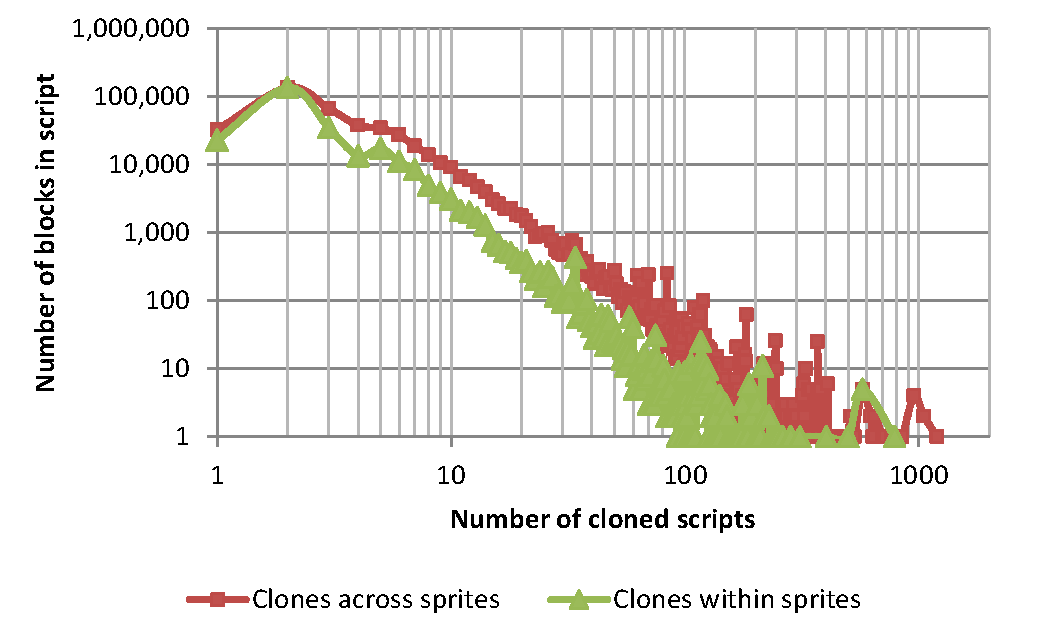
\includegraphics[width=0.45\textwidth]{fig/charts/11cloneslines}
	\caption{Number of cloned scripts of different block sizes across and within sprites}
	\label{fig:cloneslines}
\end{figure}

To examine the long method and the large class smells, we consider them in the context of Scratch as large script and large sprite smells respectively. For these two smells we use the number of blocks as the size metric. Figure \ref{fig:longmethod} presents the number of blocks in the scripts and the sprites of our dataset. We used these numbers to split the dataset and retrieve the top 10\% largest scripts and sprites, as is commonly done in both source code analysis~\cite{alves_deriving_2010} and analysis of end-user programming artifacts like spreadsheets~\cite{hermans2015detecting}. Using that strategy, we set the thresholds for the calculation of the large script and large sprite: it is 18 blocks and 59 blocks respectively. The results we obtained using these thresholds are presented in Section \ref{RQ3}.

\begin{figure}
	\centering
	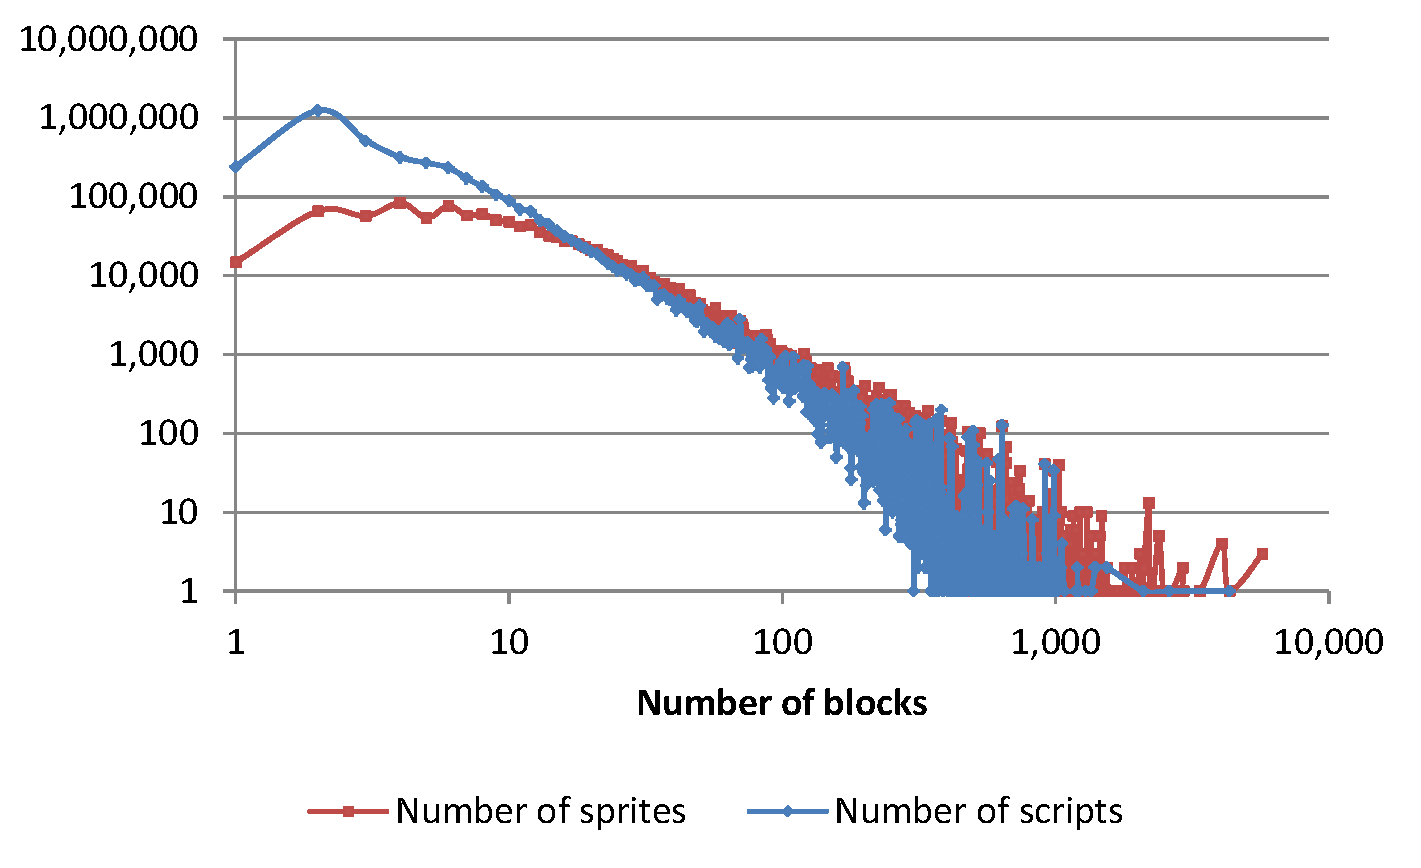
\includegraphics[width=0.45\textwidth]{fig/charts/13longmethod}
	\caption{Size of sprites and scripts in number of blocks}
	\label{fig:longmethod}
\end{figure}

\section{Results}
\label{sec:results}
In the following sections, for each of the research questions, we describe the results obtained through the analysis of the  \nAnalyzedPrograms~Scratch projects in our dataset.

\subsection{Program Size and Complexity}
\label{RQ1}
The dataset contains a relatively small number of projects without any code: \nemptyPrograms~ (5.77\%). Through random manual sampling we found that in some cases these projects contains only sprites and costumes, but no code, while in other projects they were entirety empty apart from the Scratch cat added by default. Since these projects are empty in terms of code we excluded them from further analysis, leaving the final number of analyzed non-empty projects to \nScriptPrograms.

\begin{table*}[ht]
	\centering
	\begin{tabular}{llrrrrrr}
		&&\textbf{mean}&\textbf{min}&\textbf{Q1}&\textbf{median}&\textbf{Q3}&\textbf{max}\\
		\hline
		Size&Sprites with code per project&5.68&1&1&2&5&525\\
		&Scripts per project&17.35&1&2&5&12&3,038\\
		&Number of blocks per project&154.55&1&12&29&76&34,622\\
		&Blocks in Stage per project&4.80&0&0&0&3&2,613\\
		&Blocks in Sprites per project&115.57&0&10&26&68&34,613\\
		&Blocks in Procedures per project&34.17&0&0&0&0&20,552\\
		\hline
		Complexity&McCabe Cyclomatic Complexity (CC) per script&1.58&1&1&1&1&246\\
		&McCabe CC per procedure script&3.75&1&1&2&4&183\\
		\hline
		Procedures&Procedures per project with procedures&11.50&1&1&2&6&847\\
		&Arguments per Procedure&0.95&0&0&0&1&53\\
		&Numerical arguments per procedure with arguments&1.73&0&1&1&2&22\\
		&Text arguments per procedure with arguments&0.28&0&0&0&1&24\\
		&Boolean arguments per procedure with arguments&0.13&0&0&0&0&14\\
		&Calls per procedure&2.14&0&1&1&2&526\\
		&Scripts with calls per procedure&1.13&0&1&1&1&59\\
		\hline
		Programming&Variables per project&2.06&0&0&0&1&340\\
		concepts&Scripts utilizing variable&4.97&1&1&3&5&1,127\\
		&Lists per project&0.55&0&0&0&0&319\\
		&Conditional statements per project&10.02&0&0&0&3&5,950\\
		&Loop statements per project&7.65&0&1&2&5&2,503\\
		&User input blocks per project&4.77&0&0&1&4&1,889\\
		&Broadcast-receive statements per project&8.57&0&0&0&2&2,460\\	
		\hline
	\end{tabular}
	\caption{Summary statistics from the dataset of \nScriptPrograms~non-empty Scratch projects}
	\label{tbl-size}
\end{table*}

\begin{table}[ht]
	\centering
	\begin{tabular}{lrr}
		\hline
		&\textbf{Number of}&\\
		&\textbf{projects}& \textbf{\%}\\
		\hline
		Retrieved & 250,166 & \\
		Analyzed & 247,798 & \\
		Non-empty (used for statistics) & \textbf{233,491} & \\
		\hline
		\textit{Projects with:} & & \\

		Procedures & 17,979 & 7.70\%\\
		Recursive procedures &  1,052 & 0.45\%\\
		Variables & 73,577 & 31.51\% \\
		Lists & 9,358 & 4.01\% \\
		Conditional statements & 92,959 & 39.81\% \\
		User input blocks& 131,314 & 56.24\% \\
		Loop statements & 180,210 & 77.18\% \\
		\texttt{repeat until <condition>} & 31,739 & 13.59\% \\
		\texttt{broadcast} - \texttt{receive} & 69,039 & 29.57\%\\
		Cloned scripts across sprites & 59,634 & 25.54\% \\
		Cloned scripts within sprites & 23,671 & 10.14\%\\
		Cloned procedures & 4,945 & 2.12\%\\
		Cloned blocks across sprites & 60,554 & 25.93\%\\
		Exact clones across sprites & 27,574 & 11.81\%\\
		Exact clones within sprites & 2,043 & 0.87\%\\
		Dead code & 65,760 & 28.16\%\\
		Large scripts & 69,521 & 29.77\%\\
		Large sprites & 31,954 & 13.68\%\\		
		\hline
	\end{tabular}
	\caption{Elements and characteristics of the projects in the dataset}
	\label{tbl-characteristics}
\end{table}

\begin{figure}
	\centering
	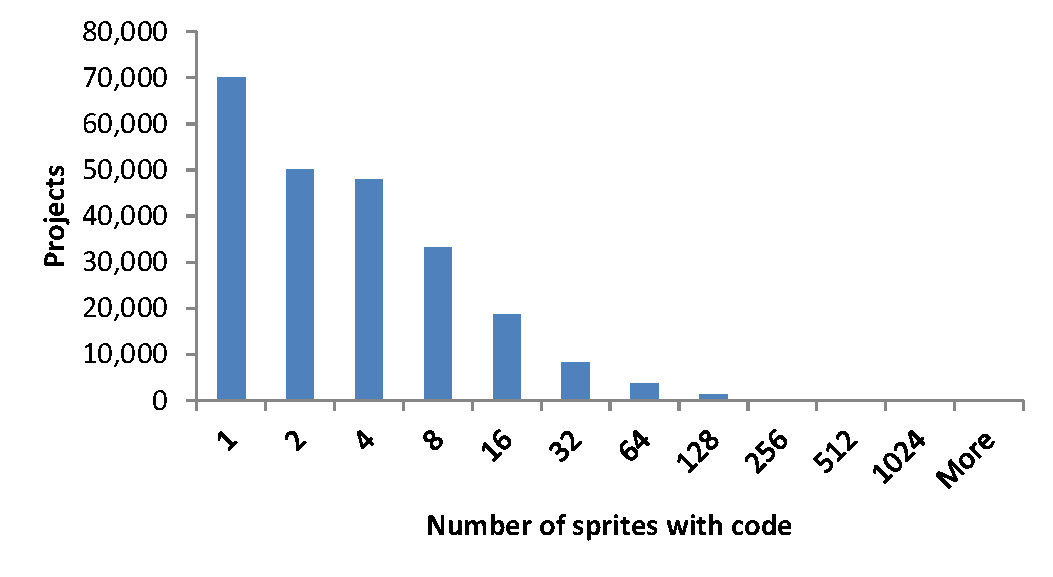
\includegraphics[width=0.45\textwidth]{fig/charts/1sprites}
	\caption{Number of sprites in the analyzed projects}
	\label{fig:size-sprites}
\end{figure}
\begin{figure}
	\centering
	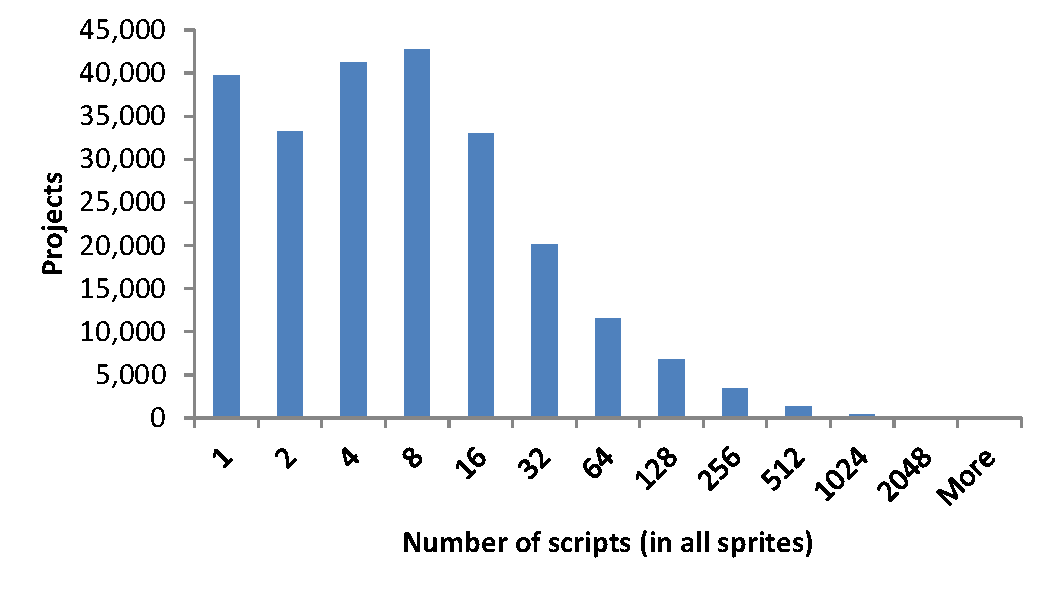
\includegraphics[width=0.45\textwidth]{fig/charts/1scripts}
	\caption{Number of scripts in the analyzed projects}
	\label{fig:size-scripts}
\end{figure}
\begin{figure}
	\centering
	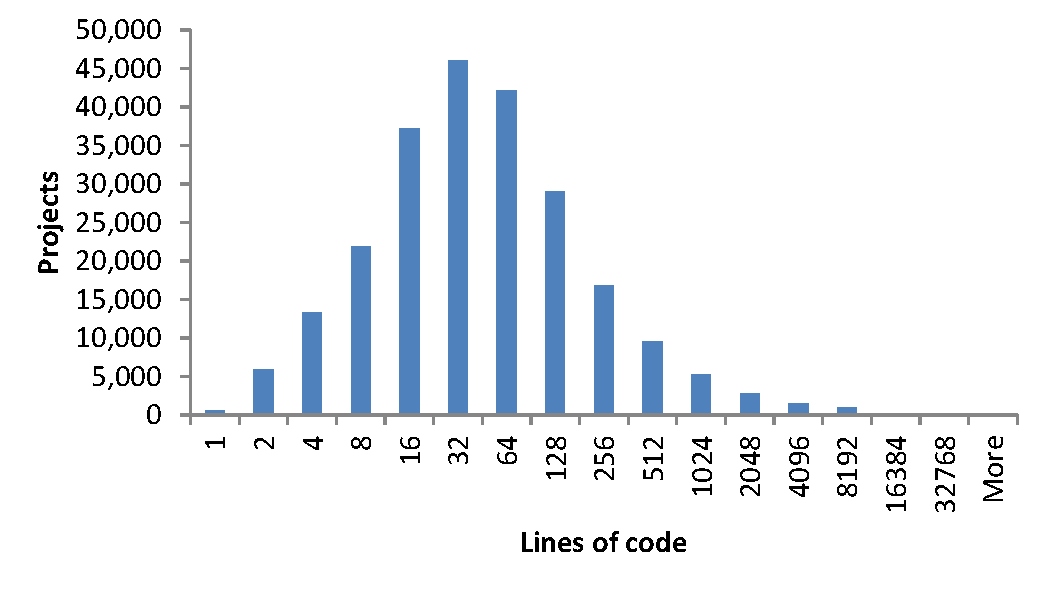
\includegraphics[width=0.45\textwidth]{fig/charts/1locs}
	\caption{Number of blocks in the analyzed projects}
	\label{fig:size-locs}
\end{figure}
\begin{figure}
	\centering
	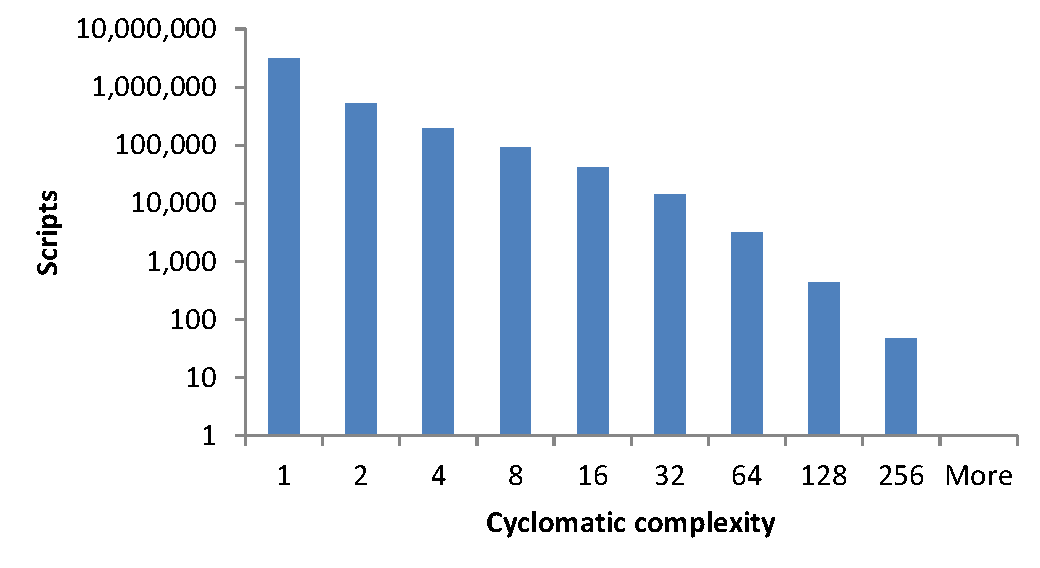
\includegraphics[width=0.45\textwidth]{fig/charts/3cyclomatic}
	\caption{McCabe cyclomatic complexity of the \nscripts~analyzed scripts}
	\label{fig:cyclomatic}
\end{figure}


In Table \ref{tbl-size} we summarize the statistics for the analyzed metrics. We use the mean value and the five-number summary to describe the dataset in terms of the number of sprites with code per project (including the stage sprite) and the number of scripts and blocks per project. Figures \ref{fig:size-sprites}, \ref{fig:size-scripts}, \ref{fig:size-locs} and plot the distribution of these size metrics.

We find that the majority of Scratch projects are small; 75\% of the projects have up to 5 sprites, 12 scripts and 76 blocks, while one fourth of the projects have up to 12 blocks. On the other end, 5\% of the projects (11,712) have more than 18 sprites and 4.8\% (11,214) consist of more than 500 blocks. The analysis also highlighted some surprisingly large projects: 135 with more than 300 sprites and even 30 projects with more than 20,000 blocks, whose Scratch identifiers are made available for further inspection.\footnotemark[\ref{repo}]

The number of blocks metric was further analyzed to understand code organization. As shown in Table \ref{tbl-size}, the majority of Scratch code---74.78\% out of \nLOC~blocks---is written within sprites. An additional 3.1\% of the total blocks are found in the stage class. More interestingly, the remaining 22.11\% are blocks within defined procedures, which are found in only 7.7\% (17,979) of the projects. The projects that contain procedures use them a lot; almost half of their total blocks (48.81\%) are within procedures.

We further analyzed the utilization frequency of the different block shapes and categories, as defined in the Scratch documentation. Figures \ref{fig:categories} and \ref{fig:shapes} present the results in terms of number of blocks from the total \nLOC~blocks in the dataset projects. The most commonly used blocks are from the Control and Data categories. The Others category includes the blocks related to procedure calls and arguments.

\begin{figure}
	\centering
	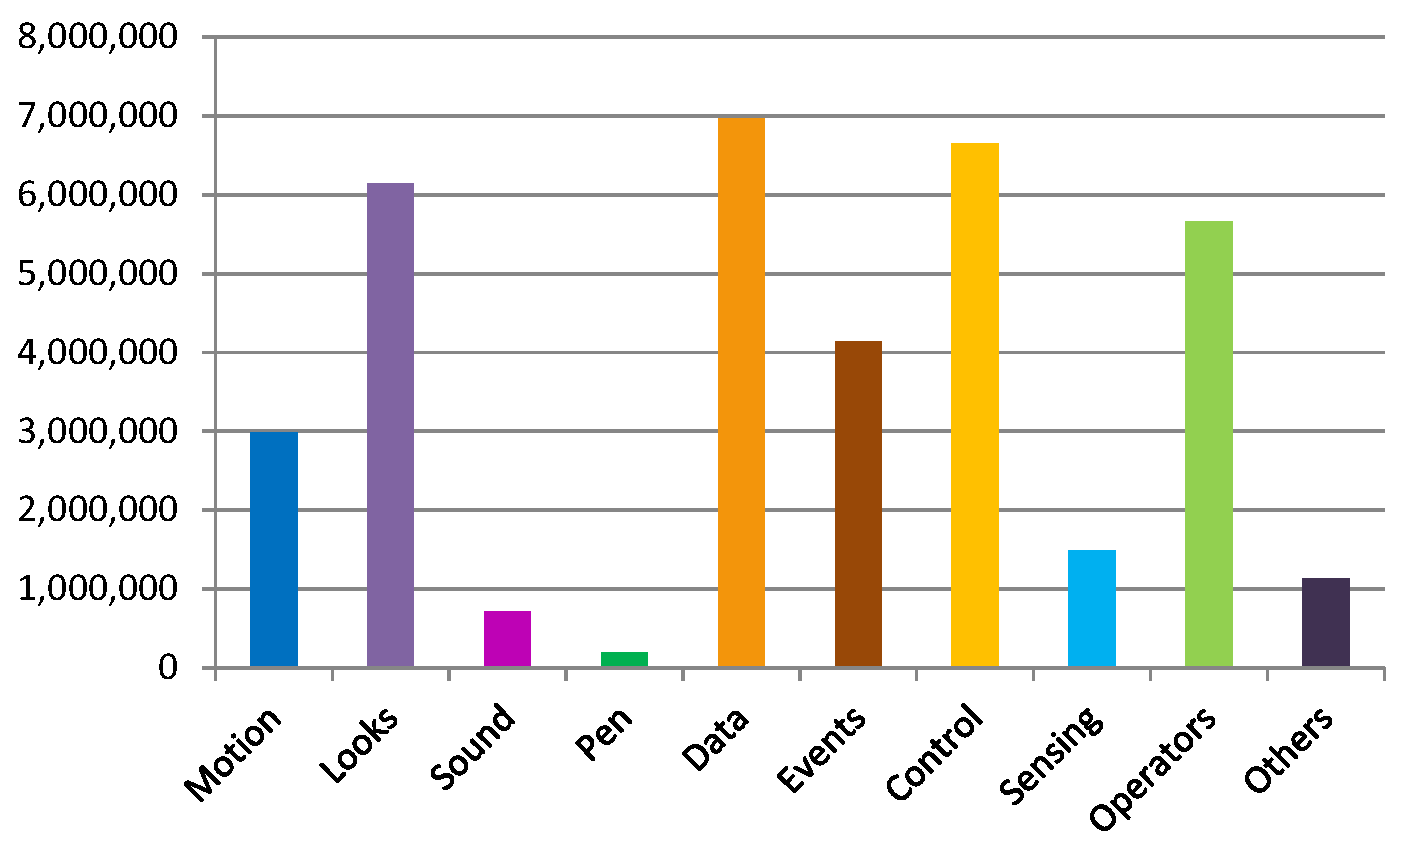
\includegraphics[width=0.45\textwidth]{fig/charts/16Categories}
	\caption{Number of blocks from each category in the analyzed projects}
	\label{fig:categories}
\end{figure}
\begin{figure}
	\centering
	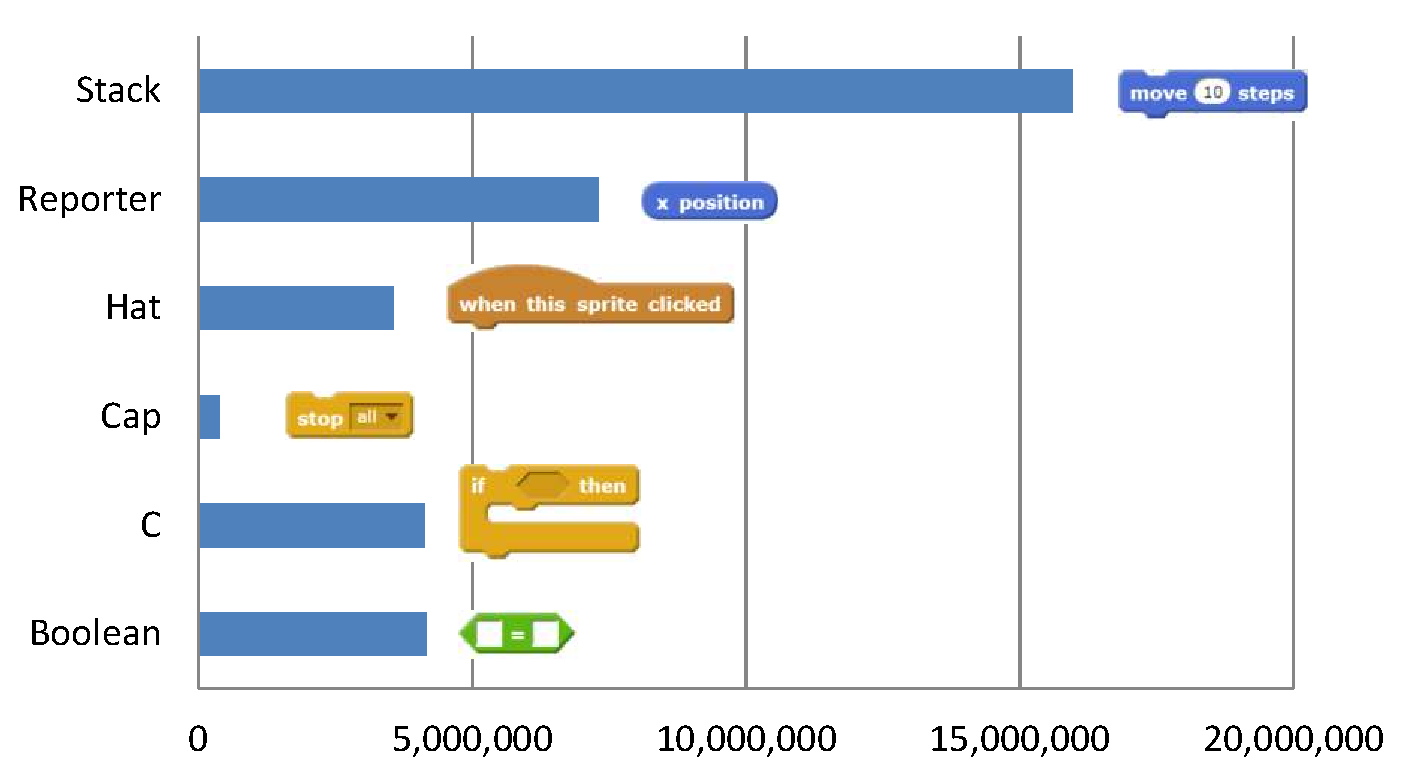
\includegraphics[width=0.45\textwidth]{fig/charts/16Shapes}
	\caption{Number of blocks of each shape in the analyzed projects}
	\label{fig:shapes}
\end{figure}

To understand the complexity of the Scratch projects in our dataset, we use the McCabe cyclomatic complexity. The results of this metric per script are plotted in Figure \ref{fig:cyclomatic}. The majority (78.33\%) of \nscripts~scripts contain no decision points, while 13.08\% have a cyclomatic complexity of 2, containing exactly one decision point. The complexity is higher, over 4, for 3.67\% of the scripts. The analysis also highlighted 209 scripts with a cyclomatic complexity over 100 and up to 246.\footnotemark[\ref{repo}] Cyclomatic complexity was greater (mean value of 3.32\%) in defined procedures, with 56.46\% of the procedures having at least one decision point.

\noindent
\fbox{
	\begin{minipage}{0.46\textwidth}
		RQ1: The majority of Scratch projects are small and simple; 75\% of the projects have up to 5 sprites, 12 scripts, 76 blocks and no decision points. Most code is written in sprites. A small number of projects (7.7\%) use procedures, but they use them a lot and for more complex code. There exist surprisingly large and complex projects.
	\end{minipage}}

\subsection{Programming Abstractions and Concepts}
\label{RQ2}
The first method for abstraction that we investigate are procedures. In the dataset we found 206,799 procedures in 17,979 (7.7\%) projects. As summarized in Table \ref{tbl-size}, the projects that contain procedures have an average of 11.5 procedures, but with 53.59\% of these projects having up to 2. Figure \ref{fig:proceduresperproject} shows the distribution of procedures in projects. Regarding procedure arguments, we found that 55.57\% have no arguments and 19.48\% have only one (shown in Figure \ref{fig:procedurearguments}). The majority of procedure arguments (80.59\%) are numeric, and the least used argument type is the boolean one---6.23\% of the total procedure arguments, found in 5.32\% of the procedures.

\begin{figure}
	\centering
	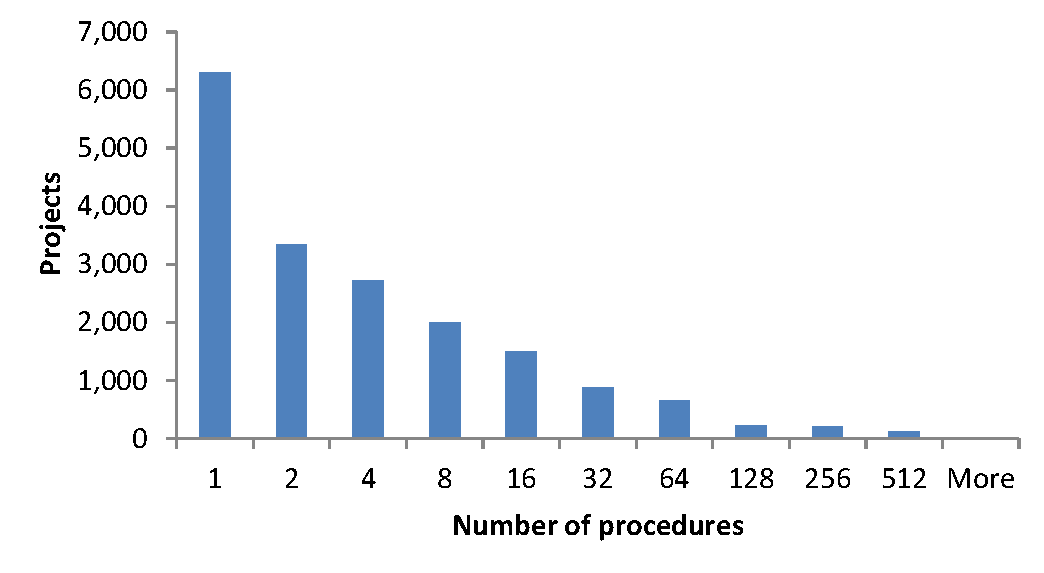
\includegraphics[width=0.45\textwidth]{fig/charts/6proceduresperproject}
	\caption{Number of procedures for the 17,979 projects that include at least one}
	\label{fig:proceduresperproject}
\end{figure}

\begin{figure}
	\centering
	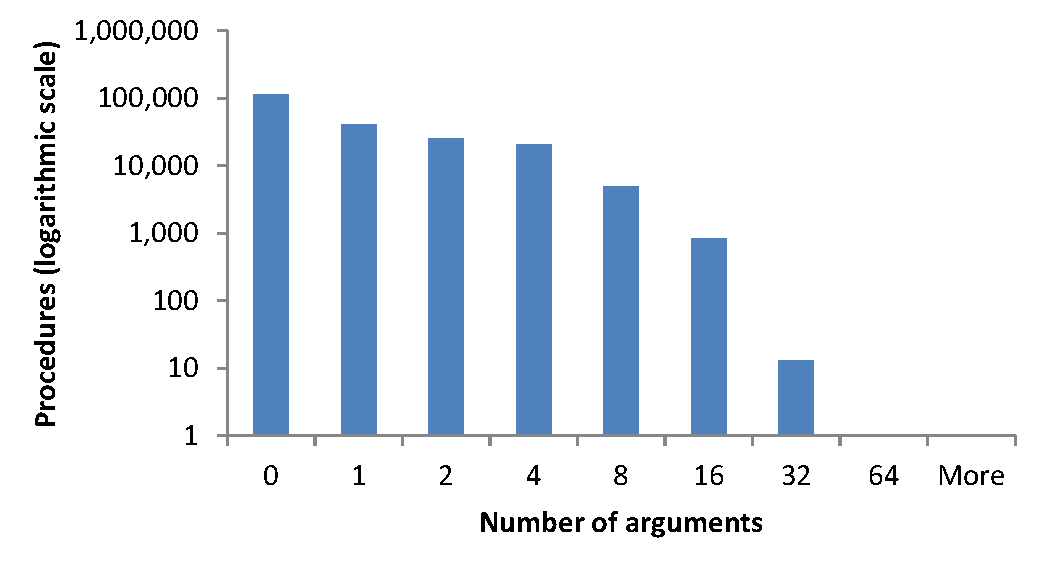
\includegraphics[width=0.45\textwidth]{fig/charts/5arguments}
	\caption{Number of arguments for the procedures in the dataset}
	\label{fig:procedurearguments}
\end{figure}

The use of procedures in projects was further investigated through the procedure calls, summarized in Figure \ref{fig:procedurecalls}. Most procedures are called exactly once (62.32\% of them) or twice (14.30\%) and from exactly one script (85.92\% of them). Examining the origin of procedure calls, we observed that most of the calls (56.09\%) originate from other procedures, and even 1.06\% originate from the same procedure, making them recursive calls. These recursive procedures are found in 1,052 projects, whose identifiers are made available.\footnotemark[\ref{repo}]

\begin{figure}
	\centering
	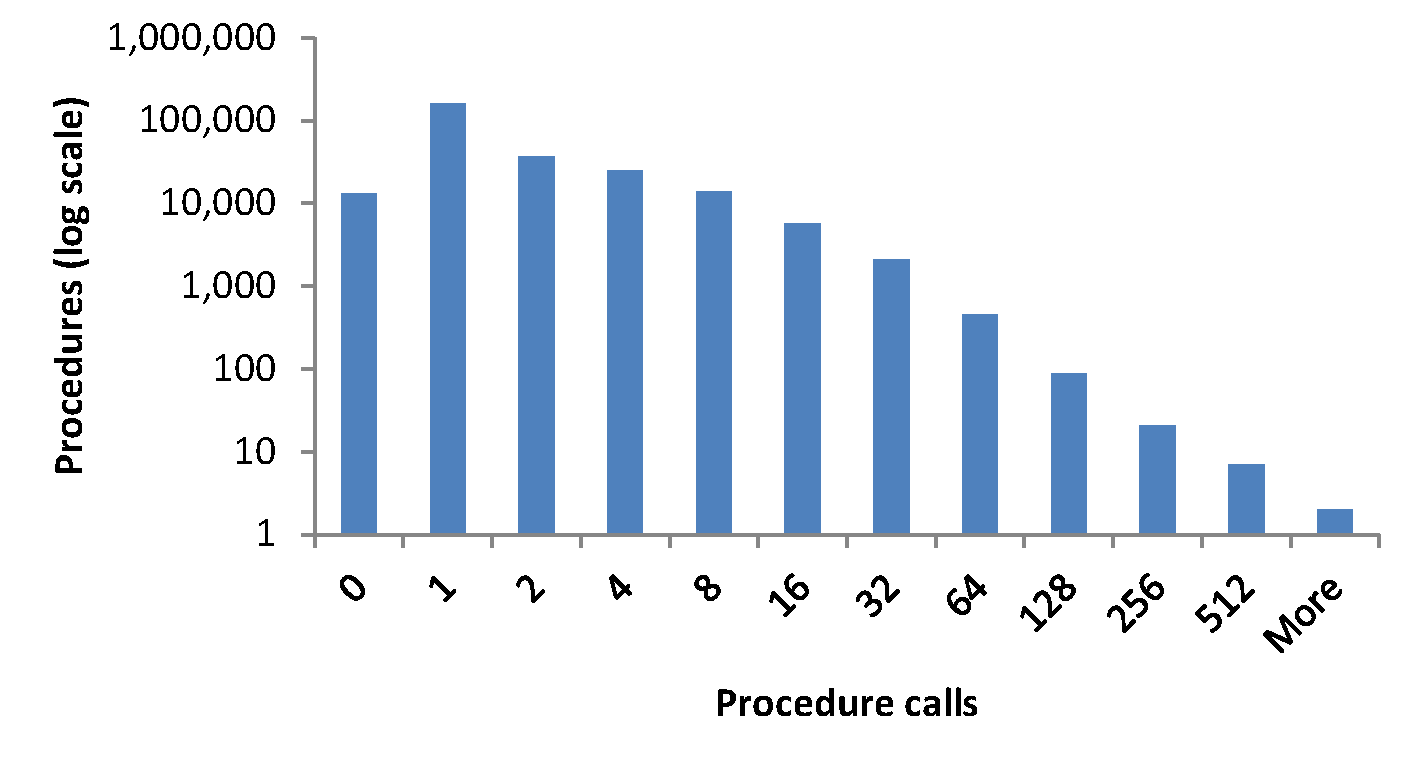
\includegraphics[width=0.45\textwidth]{fig/charts/7procedurecalls}
	\caption{Number of calls of each procedure in the dataset}
	\label{fig:procedurecalls}
\end{figure}

As shown in Table \ref{tbl-characteristics}, almost one-third of the projects use variables and a small number (4.01\%) use lists. The number of variables that is being used is also limited, with only 7.48\% of the projects having 5 or more variables. The distribution of variable and list utilization is shown in Figure \ref{fig:variables}. Exceptional cases exist: the analysis highlighted 842 projects with more than 100 variables and with a maximum of 340. Examining the initialization of variables through the \texttt{set <variable> to <value>} blocks, we found that for 4.83\% of all variables this was missing. While failing to initialize a variable in Scratch will not result in a runtime error as in some other programming languages, correctly setting the initial state of the program is important \cite{boe_hairball:_2013}.

%commented by Felienne: 1) this is not really scope and 2) we cannot distinguish, so why mention it?
%The scope of variables was also analyzed: As shown in Table \ref{tbl-size}, each variable is used by an average of 4.97 different scripts, with a median value of 3. However, we must note that this measurement might not be entirely accurate, because variables might be defined in the scope of specific sprites. With our dataset we cannot differentiate global from local variables and we would consider local variables defined with the same name in different sprites as global variables.

\begin{figure}
	\centering
	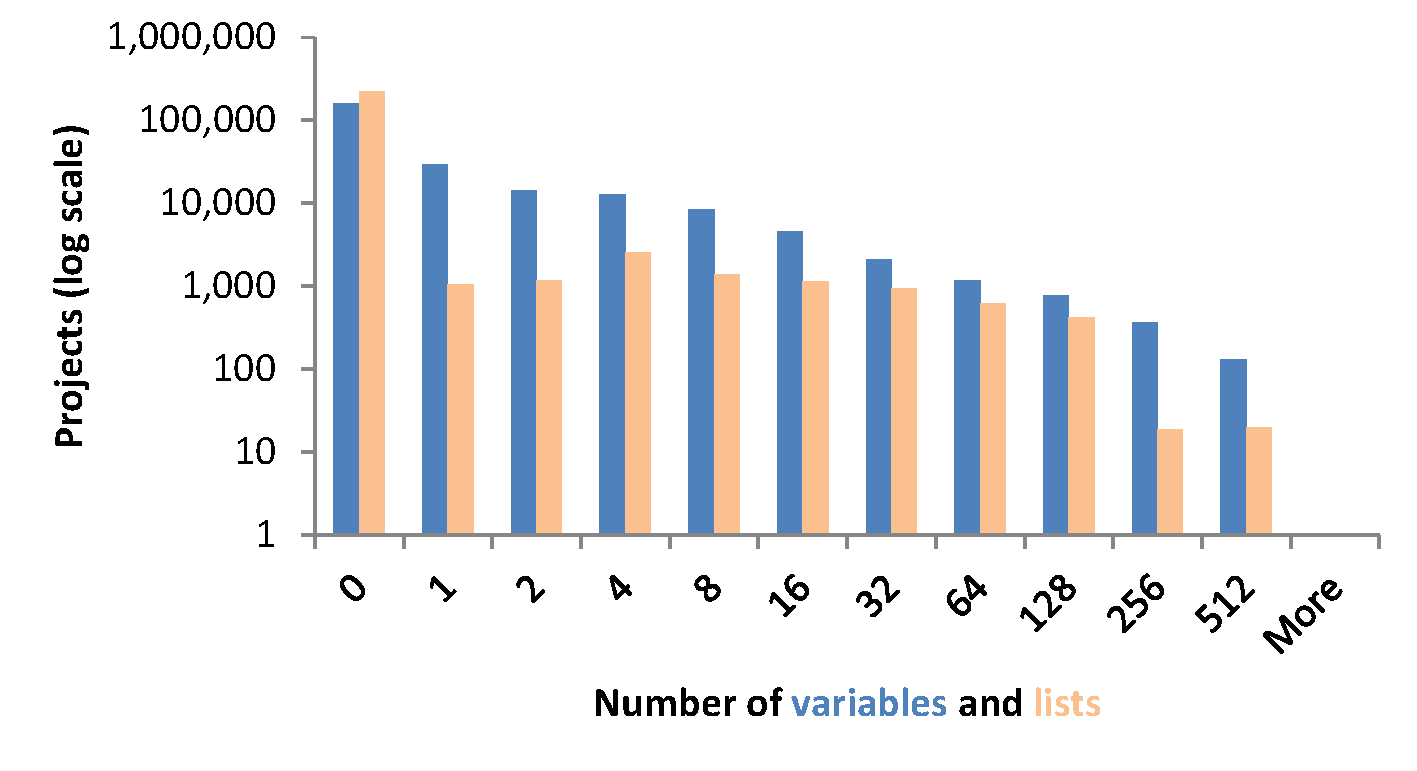
\includegraphics[width=0.45\textwidth]{fig/charts/8variableslists}
	\caption{Number of variables and lists used in the projects}
	\label{fig:variables}
\end{figure}

Regarding program control features, conditional statements (blocks \texttt{if <condition> then} and \texttt{if <condition> then else}) are used by 39.81\% of the projects. Loops (blocks \texttt{repeat <times>}, \texttt{forever} and \texttt{repeat until <condition>}) are more common, used by 77.18\% of the projects. The most common of the three is the \texttt{forever} block, accounting for 51.86\% of all loops and the least common one is the \texttt{repeat until <condition>} block, accounting for 11.57\% and used in 13.59\% of the total projects.
	
Investigating user interactivity functionality, we found that 56.24\% of the projects in the dataset contain user input blocks---an average of 8.48 blocks per such project. Table \ref{tbl-userinput} lists the frequency of use of user input controls. We do not include the \texttt{when Green flag pressed} block here, as this is just used to start a Scratch program and hence cannot really be considered input into the program. The most commonly used user input block is the \texttt{when key pressed}, found in 71,096 (30.45\% of the total) projects. The most frequently used parameter for the \texttt{key} attribute is the space key, followed by the arrows and then the letters and numbers.

\begin{table}
	\centering
	\begin{tabular}{lrr}
		\hline
		\textbf{Block}&\textbf{Projects}&\textbf{Occurrences}\\
		\hline
	\texttt{when <> key pressed}&71,096&294,771\\
	\texttt{when this sprite clicked}&39,179&198,342\\
	(Sensing) \texttt{key <> pressed?}&37,919&291,657\\
	(Sensing) \texttt{ask <> and wait}&19,039&66,850\\
	(Sensing) \texttt{mouse down?}&9,115&54,079\\
	(Sensing) \texttt{<attrib> of <>}&9,068&155,468\\
	(Sensing) \texttt{mouse X}&5,977&27,321\\
	(Sensing) \texttt{mouse Y}&3,940&22,035\\
	\texttt{when <sensor> > <value>}&705&1,570\\
	(Sensing) \texttt{video <> on <>}&434&1,397\\
		\hline
	\end{tabular}
	\caption{Frequency of use of user input blocks in the \nScriptPrograms~projects of the dataset}
	\label{tbl-userinput}
\end{table}

Users can define their own events, using the blocks \texttt{broadcast}, \texttt{broadcast and wait} and \texttt{when I receive}.These blocks are used by 29.57\% of the projects. \texttt{broadcast and wait} is rarely used, in only 3.87\% of the projects.

%user interativity		
\noindent
\fbox{
	\begin{minipage}{0.46\textwidth}
RQ2: One third of the projects use variables, sometimes without initializing them. 39.81\% of the projects contain conditional statements and 77.18\% contain loops, but conditional loops are rarely used. More than half of the projects are interactive. 29.57\% of the projects use broadcast and receive blocks. Most procedures are called once or twice, from a single script which, in more than half of the cases, is another procedure. Recursive procedure calls exist in 1,052 (0.45\% of the total) projects.
	\end{minipage}
}


\subsection{Code smells}
\label{RQ3}
The duplicated code smell is the first smell that we examine. As explained in Section \ref{dataAnalysis}, we use 5 as the minimum number of blocks for the identified clones. In total, in the dataset we found 170,532 scripts cloned across sprites in 59,634 (25.54\% of the total non-empty) projects. 726,316 copies of these scripts were found, making each clone being copied an average of 4.26 times. Figure \ref{fig:clonesprojects} plots the distribution of clones across projects. The majority of projects contain up to two cloned scripts; 7.24\% of the projects contain three or more. Figure \ref{fig:clonescopies} plots the number of copies of the identified clones. It is of interest that 79,378 (46.55\%) of the identified clones are copied three or more times, and even in 585 cases from 411 projects they are copied more than 50 times and up to 974.\footnotemark[\ref{repo}]

\begin{figure}
	\centering
	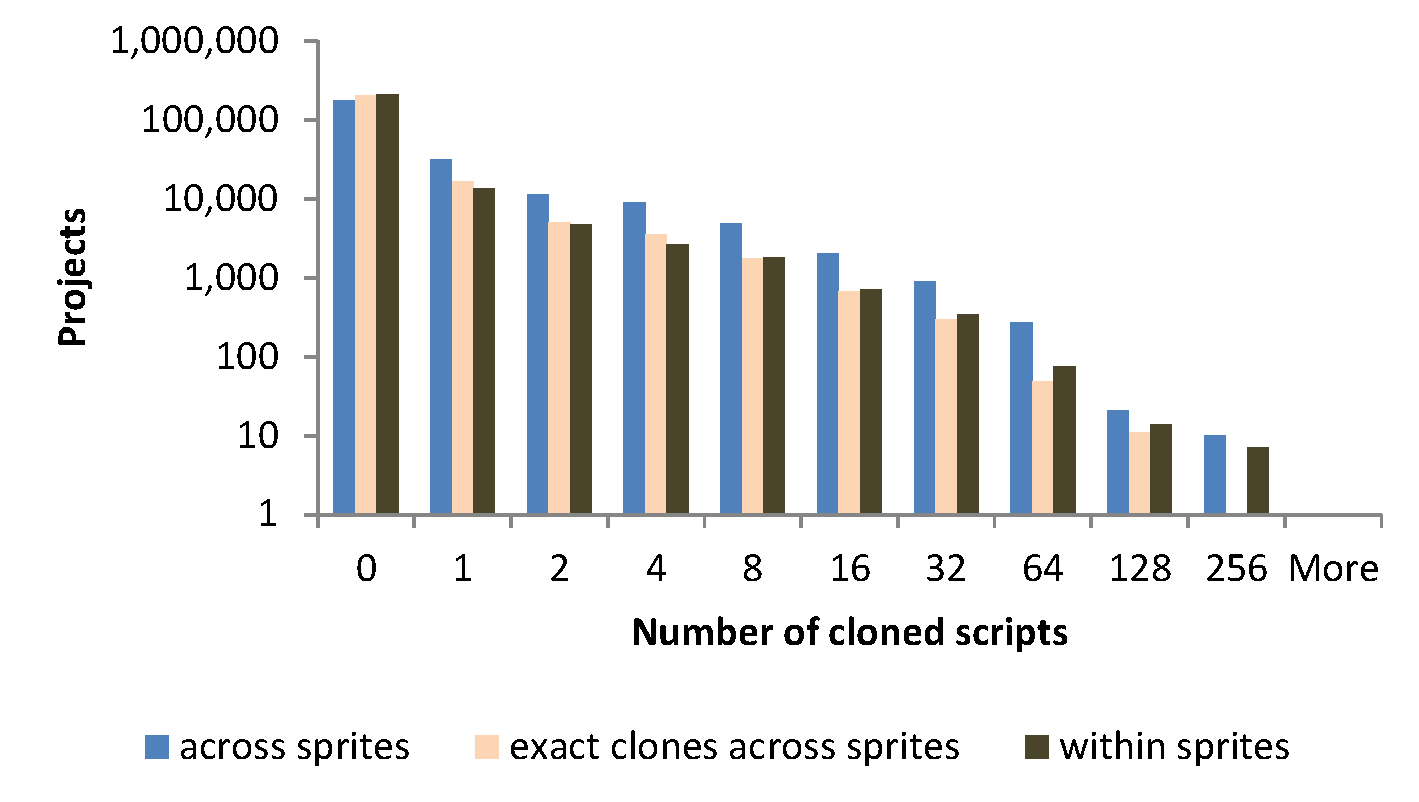
\includegraphics[width=0.45\textwidth]{fig/charts/11clonesprojects}
	\caption{Cloned scripts in the dataset projects}
	\label{fig:clonesprojects}
\end{figure}

\begin{figure}
	\centering
	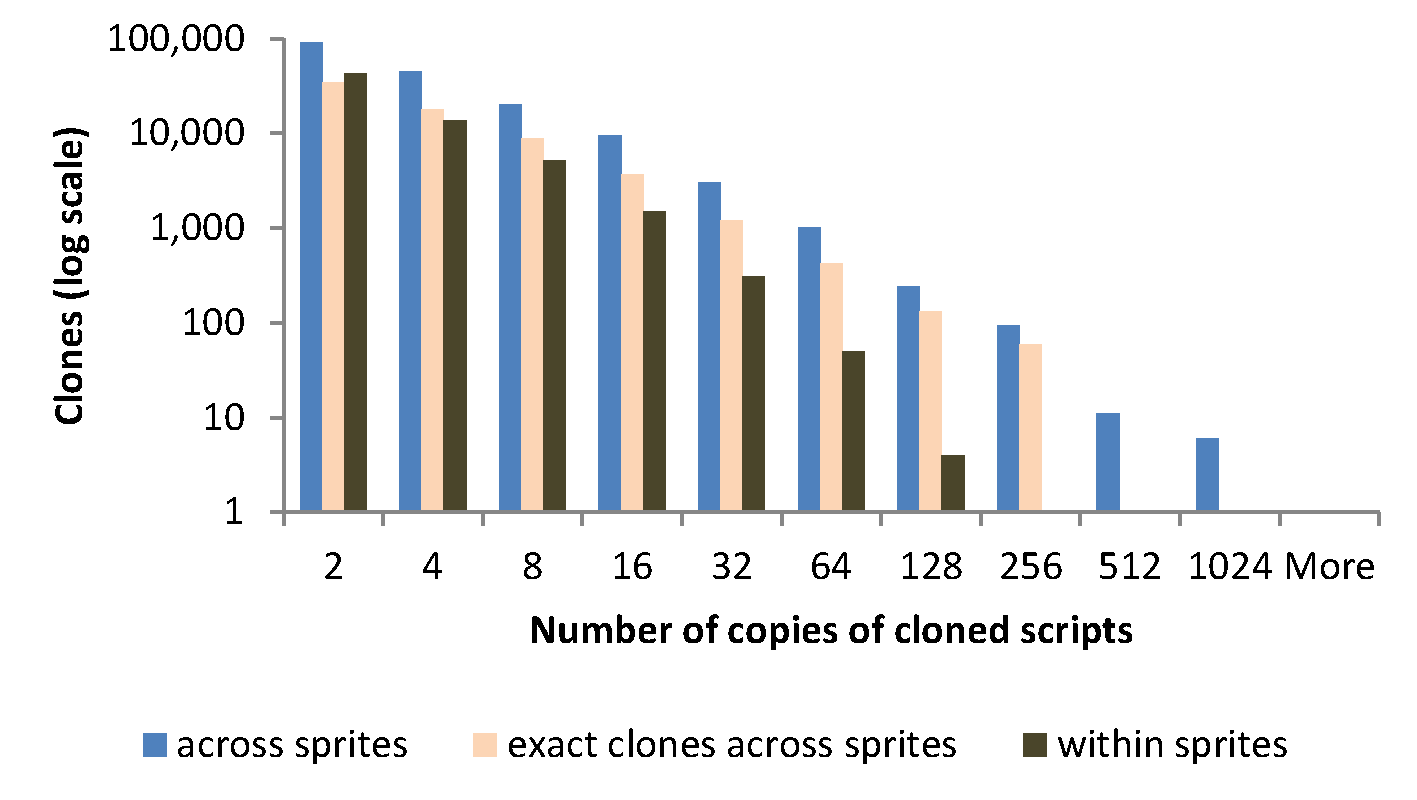
\includegraphics[width=0.45\textwidth]{fig/charts/11clonescopies}
	\caption{Number of copies of the identified clones}
	\label{fig:clonescopies}
\end{figure}

We further inspected which of the identified clones were duplicated only within the same sprite: 63,682 (37.34\% of the total) clones, in 10.14\% of all projects. Procedure clones were measured to 12,878 (7.55\% of the total) clones, in 2.12\% of the projects.

Exact clones were found in 11.81\% of the total projects. Their total number was 66,750 (39.14\% of the total) clones. Exact clones in the same sprite are cases of clearly redundant code. These were rare, found in only 0.87\% of the projects.

Apart from whole scripts we also examined cases where scripts differed only in the first (Hat) block. This way we examine if Scratch programmers assign the same functionality to handle different types of events. Cloned functionality blocks are found to be rare: without considering the first block, only 2,243 additional clones were found in 920 projects.

The second smell that we examine is the dead code smell. We identify four types of dead code: (1) procedures that are not invoked, (2) unmatched broadcast-receive messages, (3) code that is not invoked and (4) empty event scripts. Investigating the first type, we find that a significant number of the defined procedures (13,036 or 5.06\%) are not called in the projects. This is also shown in Figure \ref{fig:procedurecalls} and it occurs in 2,079 projects. For the second type, we examined the broadcast-receive messages and found that they are not always synchronized: 3,33\% of the \texttt{when I receive} blocks were found to wait for a message that is never being broadcasted, while 4,4\% of the \texttt{broadcast} blocks broadcast a message that is not being received. This lack of syncronization occurs in 18,669 (7.99\% of the total) projects.

The third and fourth cases are incomplete scripts. They are either never invoked due to the lack of a starting \texttt{when <trigger>} block from the Scratch Events or Control category, or are comprised of only a \texttt{when <trigger>} block without any functionality. A total of 322,475 scripts like that were found in 56,890 (24.36\% of the total) projects. The majority of these scripts (86.6\%) are scripts missing the starting block. Examining the size of these dead scripts, 72.34\% are composed of a single block. As shown in Figure \ref{fig:deadcode}, however, considerably large dead scripts exist; 2,358 of these scripts originating from 1,553 different projects have more than 30 blocks and up to 2,610.\footnotemark[\ref{repo}]

The number of projects exhibiting the dead code smell, considering all four types of dead code combined, is 65,760 (28.16\% of the total projects).

\begin{figure}
	\centering
	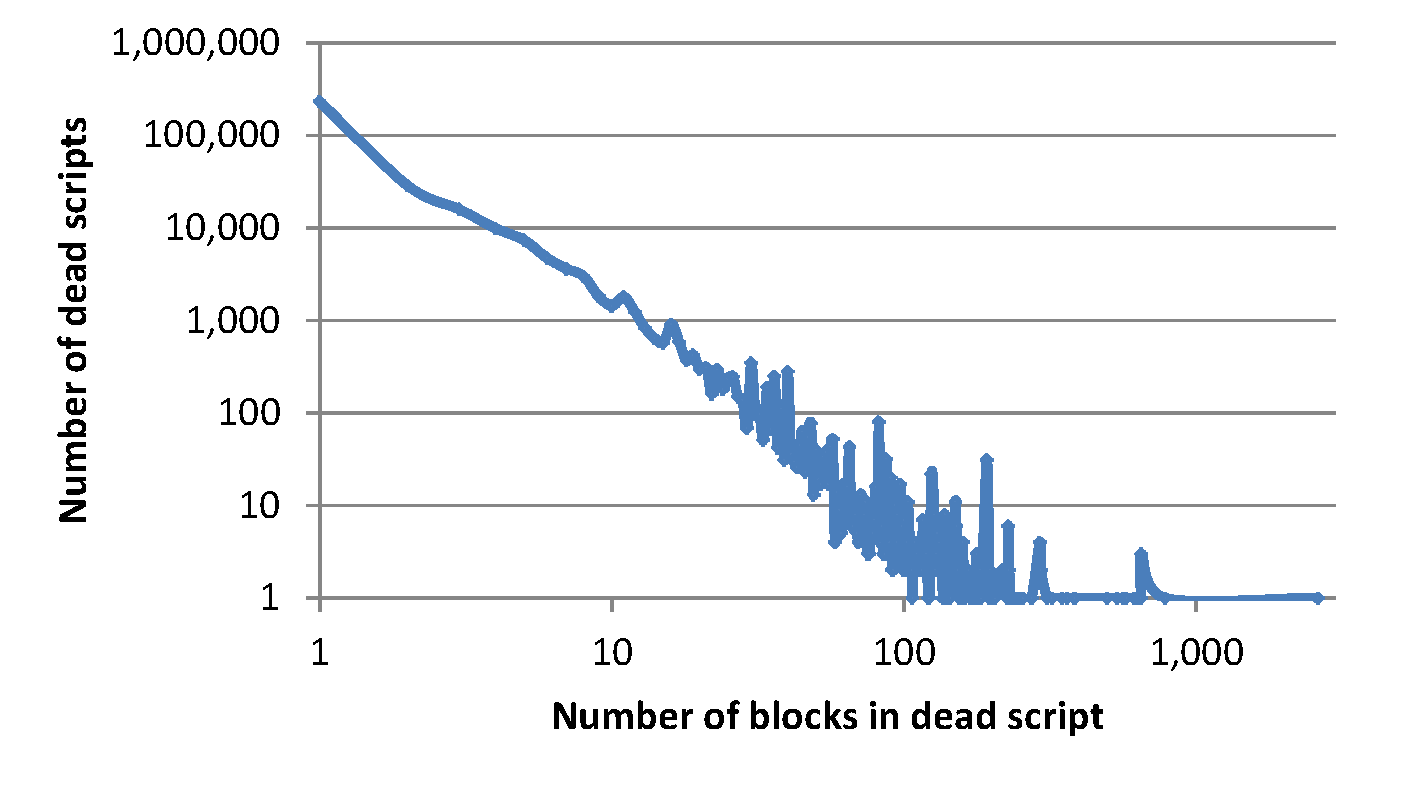
\includegraphics[width=0.45\textwidth]{fig/charts/12deadcode}
	\caption{Size of scripts identified as dead code}
	\label{fig:deadcode}
\end{figure}

Finally, we examine the large script and the large sprite smells. The thresholds we use for the identification of large scripts and large sprites are 18 blocks and 59 blocks respectively, as explained in Section \ref{dataAnalysis}. The number of projects exhibiting the large script smell, i.e., containing at least one script with 18 or more blocks, is 69,521 (29.77\% of the total projects) and the number of projects with the large sprite smell is 31,954 (13.68\%).

\noindent
\fbox{
	\begin{minipage}{0.46\textwidth}
RQ3: Code clones are found in 25.54\% of the projects, with 46.55\% of the clones copied three or more times, in the same or across sprites. 28.16\% of the projects contain code that is never invoked, and thus exhibit the dead code smell. In some cases these scripts are large. The large script smell is found in 29.77\% of the projects and the large sprite one in 13.68\%.
	\end{minipage}}


\section{Discussion}
\label{sec:discussion}
\subsection{Implications}
We believe a large scale study of programs like ours can help language designers to tailor their language. In this section we highlight directions in which our study could support language design. There are many other implications to be considered, which is why we have made our dataset public.

\subsubsection{Popularity of different block types}
Our analysis shows that some categories of blocks are rarely used, like the `Pen' blocks, of which only 194,885 occur within 19,090 (8.17\% of the total) programs. Hence, in future changes to the language, `Pen' blocks might be less important to users to support or maintain. 

\subsubsection{Dead code}
In our analysis, we find that more than one quarter of the Scratch projects contain dead `scripts': scripts that are never invoked due to the lack of a starting \texttt{when <trigger>} block from the Scratch Events or Control category, scripts that are comprised of only a \texttt{when <trigger>} block without any functionality, procedures that are not invoked, or unmatched broadcast-receive messages.

In a sense, the dead scripts are harmless, as they are not executed. However, they do cause `visual clutter' and might be distracting to novice programmers, as it might be hard to see which scripts are dead. In contrast to other visual educational languages, Scratch does not indicate scripts that are dead. LEGO Mindstorms, for example, does give the user such feedback by making unconnected blocks gray. 

Looking at the number of unconnected blocks, we hypothesize that Scratch programmers have a need for a separate workspace to store unconnected blocks temporarily. We envision that would be like the `backpack' meant to move scripts across sprites. In order to help novice programmers keep their code clean, the programming interface could actively encourage users to move unconnected blocks to that workspace when they exit the environment.

\subsubsection{Exact clones between sprites}
With occurrences in 11\% of the Scratch projects in our dataset, the use of exactly identical clones between sprites is relatively common. In a sense, the Scratch users are not to blame here, as Scratch does not support procedure calls between sprites, only within them. So in many cases there is no way to share the functionality other than by making a copy. We are not aware of the underlying rationale of the Scratch team that lead to this decision, however it seems that a large part of the Scratch users would use the functionality to call procedures between sprites.

\subsubsection{Sharing of scripts and procedures}
Investigating the use of clones between projects, we observe that there are 1,700 scripts that are used in multiple projects, sometimes as often as in 1,600 different projects. This seems to indicate that there are common patterns in Scratch projects, which means it might be very beneficial to Scratch programmers if they could not only share their projects, but also share some of their functionality, for others to use, like a library. An example of such a library could be: functions for platforming games, including the movement of a player, collision detection and the implementation of `lives'. This might empower new Scratch users to get started faster.

\subsection{Threats to validity}
A threat to the validity of this study is the fact that we did not scrape a random sample, but the most recent 250,000 projects. It could be the case that the programming habits of Scratch users are changing over time. However, we counterbalanced that by using a large dataset which comprises of around 2\% of all 14 million shared Scratch projects.\footnote{\url{https://scratch.mit.edu/statistics/}}.

Furthermore we use the number of blocks in the Scratch projects as a measure for the length of a program, while this does not exactly correspond to the `length' of a program in lines, and there can be multiple Scratch blocks on one line. For example, in Figure \ref{fig:ui} the `if' and `touching' blocks are present on the same `line'. We however believe that the number of blocks is a good proxy for size, and we plan a future experiment in which we will compare `lines of Scratch code' to `number of blocks'.

\section{Related Work}
\label{sec:related}

The evaluation of block-based languages in general, and Scratch in particular, as tools for programming education has received significant research attention during the past years. A number of studies have been carried out on the understanding of programming concepts and the programming practices of novice programmers in block-based environments, on the programming skills they develop, and on the quality of Scratch programs.

For example, a study on the internalization of programming concepts with Scratch with 46 students was presented in \cite{meerbaum-salant_learning_2010}. Concepts like loops, conditional loops, message passing, initialization, variables and concurency were examined, and it was found that students had problems with the last three. In a later study with an equal set of subjects \cite{Meerbaum_habits_2011} the same authors identified two bad programming habits in Scratch, namely bottom-up development and extremely fine-grained programming. They connected the later to the reduced use of if-blocks and finite loops and the increased use of infinite loops, a finding that is verified by our study. In \cite{wilson_evaluation_2012} 29 Scratch projects created from 60 students working in groups were evaluated based on a list of criteria related to programming concepts, code organization and usability design.

Most related to our study for the second research question of programming abstractions and concepts is the work by Maloney \emph{et al.} \cite{Maloney_2008}, who analyzed 536 Scratch projects for blocks that relate to programming concepts including loops, conditional statements, variables, user interaction, synchronization, and random numbers. Compared to their findings, our investigation reveals increased use of the first three concepts, and especially variables.

The Scratch automated quality analysis tools Hairball \cite{boe_hairball:_2013} and Dr. Scratch \cite{moreno-leon_dr._2015} are also related to our work on smell detection. The Hairball Scratch extension is a lint-like static analysis tool for Scratch that can detect initialization problems and unmatched broadcast and receive blocks. In their work \cite{moreno_automatic_2014}, Moreno and Robles extended Hairball to detect two bad programming habits in Scratch: not changing the default object names and duplicating scripts, and apply them for evaluating 100 projects from the Scratch repository. The results on script duplication are substantially different than ours---we find projects with script clones to appear half as frequently. The Dr. Scratch tool \cite{moreno-leon_dr._2015} includes bad naming, code duplication and dead code identification functionality, and also evaluates Scratch projects in terms of abstraction, parallelism, logical thinking, synchronization, flow control, user interactivity and data representation.

%Also related to our research are works on code smells, initiated by the work by Fowler~\cite{fowler_refactoring:_1999}. His book gives an overview of code smells and corresponding refactorings. Fowler's work was followed by efforts focused on the automatic identification of code smells by means of metrics. Marinescu~\cite{marinescu_detecting_2001} for instance, uses metrics to identify \emph{suspect} classes: classes which could have design flaws. Alves \emph{et al.}~\cite{alves_deriving_2010} focus on a strategy to obtain thresholds for metrics from a benchmark Moha \emph{et al.}~\cite{moha_decor:_2010} designed the `DECOR' method which automatically generates a smell detection algorithms from specifications. The CCFinder tool~\cite{kamiya_ccfinder:_2002} finally, aims at detecting clones in source code, which are similar to our code duplication smell.

\section{Conclusions}
\label{sec:conclusion}
In this paper we presented a large-scale study on 247,798 projects we scraped from the Scratch repository. We analyze these projects in terms of size, complexity, application of programming abstractions and utilization of programming concepts including procedures, variables, conditional statements, loops, and broadcast-receive functionality. We find that procedures and conditional loops are not commonly used. We further investigate the presence of code smells, including code duplication, dead code, long method and large class smells. Our findings indicate that Scratch programs suffer from code smells and especially from dead code and code duplication.

In addition to the findings presented in this paper, we provide as contributions the dataset that we used for our study, as well as information on the edge cases that we found in the dataset in terms of size and number of procedures, variables, cyclomatic complexity, clones and dead code.\footnotemark[\ref{repo}]

\bibliographystyle{abbrv}
\bibliography{zotero}
\end{document}
